% IPSJ v4-1 形式の簡易テンプレート(ipsj.cls を利用)
\documentclass{ipsj}
\usepackage[dvipdfmx]{graphicx}
\usepackage{booktabs}
\usepackage{array}
\usepackage{url}

\title{GSM8Kにおけるエントロピー適応型self-consistencyサンプリングの分析}

\author{佐々木 駿・川島 英之}{shun.sasaki@keio.jp}
\affiliate{aff1}{慶應義塾大学 環境情報学部}

\begin{document}

\maketitle

\section{研究概要}
本報告は,self-consistency サンプリングを実装した再現環境を用い,算数ベンチマーク GSM8K\cite{Cobbe2021TrainingVT} に対してサンプル数を最大 $n=50$ まで拡張した再現実験の結果をまとめたものである。Self-consistency は Chain-of-Thought 推論を改善する手法として注目されており\cite{Wang2022SelfConsistencyIC},本研究ではサンプル数の増加が精度・レイテンシ・各種信頼度指標に与える影響を定量的に整理することを目的とする。

\section{実験構成}
Meta-Llama-3-8B-Instruct(HF Transformers)を用い,temperature=0.7,top-p=0.9 とした。全 8,792 問に対し固定 $n=50$ の推論を一度行い,得られた 50 本の出力から先頭 $n$ 本のみを切り出して多数決を再計算するポストホック評価を採用した。記録した主な指標はプレフィックスエントロピー,投票マージン,二番手票率,サンプル生成時間である。

\section{主な結果}
\subsection{精度とレイテンシ}
表\ref{tab:accuracy}に主要なサンプル数での厳密精度と累積レイテンシを示す。10 サンプルまでは比較的大きな改善が得られるが,20 サンプルを超えると増分は 1--2pt に留まる。加えて,図\ref{fig:accuracy_curve} にサンプル数と精度・レイテンシの関係をグラフで示す。

\begin{table}[h]
  \centering
  \caption{ポストホック再集計による精度と累積レイテンシ}
  \label{tab:accuracy}
  \begin{tabular}{@{}>{\raggedright\arraybackslash}p{2cm}cc@{}}
    \toprule
    サンプル数 $n$ & 精度 & レイテンシ [s] \\
    \midrule
    1 & 0.457 & 0.39 \\
    5 & 0.648 & 1.97 \\
    10 & 0.735 & 3.94 \\
    20 & 0.780 & 7.89 \\
    30 & 0.795 & 11.83 \\
    50 & 0.810 & 19.72 \\
    \bottomrule
  \end{tabular}
\end{table}

\begin{figure}[h]
  \centering
  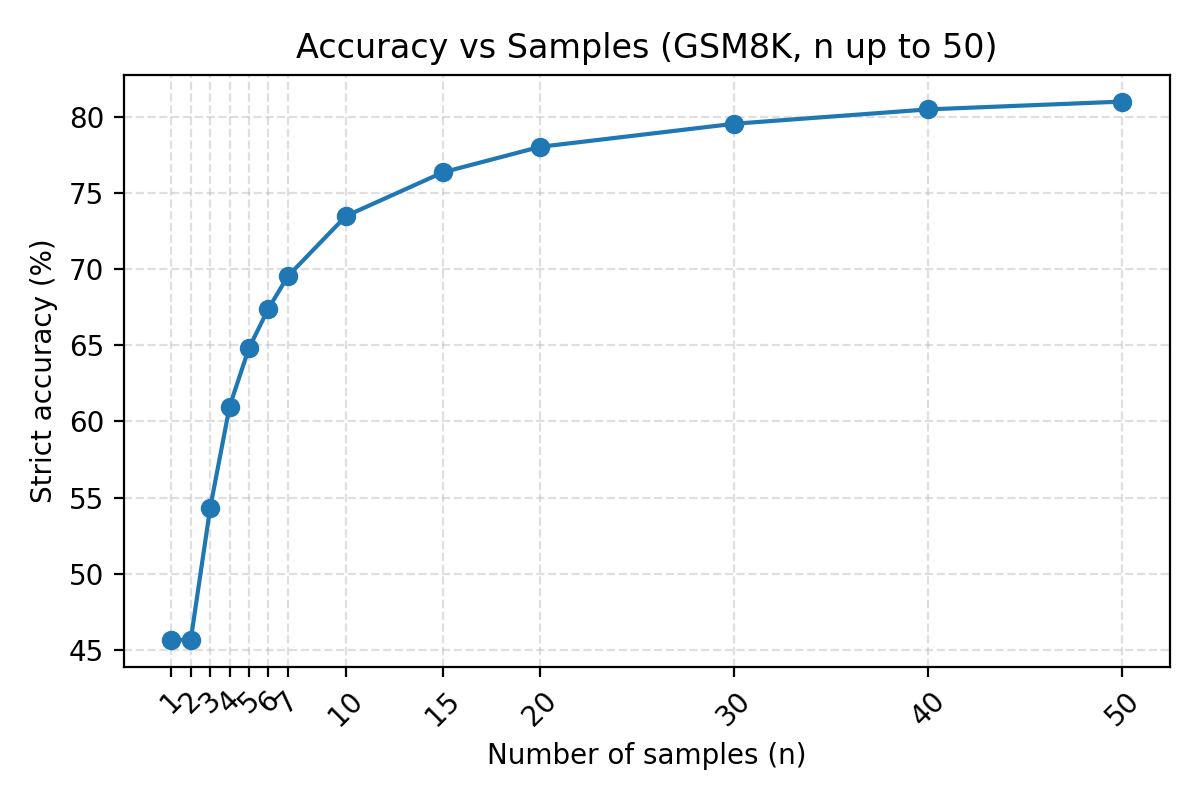
\includegraphics[width=0.8\linewidth]{../../figures/n50_batch/accuracy_vs_n50.png}
  \caption{サンプル数に対する厳密精度(上)とレイテンシ(下)の推移}
  \label{fig:accuracy_curve}
\end{figure}

\subsection{信頼度指標との相関}
表\ref{tab:correlation} に,主要指標の定義と $n=50$ 正答率との相関係数を示す。投票マージンは最も高い正の相関($r=0.37$)を示し,二番手票率は負の相関($r=-0.16$)を示した。プレフィックスエントロピーは $r=0.08$ と弱く,単独では難問検出に十分ではない。またサンプル生成時間は $r=-0.10$ であり,長時間を要する問題ほど誤答率が高い傾向が確認できた。

\begin{table}[h]
  \centering
  \caption{正答率と指標の相関(全 8,792 問)}
  \label{tab:correlation}
  \begin{tabular}{@{}p{3cm}p{6cm}c@{}}
    \toprule
    指標 & 説明 & 相関係数 \\
    \midrule
    投票マージン & 最多数回答の得票比率(0.5 で僅差,1.0 で全会一致) & $+0.37$ \\
    二番手票率 & 準多数回答の得票比率(高いほど票が割れている) & $-0.16$ \\
    プレフィックスエントロピー & 先頭 $K$ トークンの平均エントロピー & $+0.08$ \\
    サンプル生成時間 & 50 サンプル生成に要した総時間 & $-0.10$ \\
  \bottomrule
  \end{tabular}
\end{table}

\section{考察と今後の課題}
サンプル数を増やすほど安定に正解へ収束するが,$n=50$ でも 13.9\% は誤答のままであり,投票マージンが小さい問題に集中している。今後は
\begin{itemize}
  \item 投票マージンや二番手票率に基づく動的な打ち切り戦略の設計
  \item ログ尤度や自己検証プロンプトなど追加指標との統合
  \item 他データセット(MATH 等)への適用と比較
\end{itemize}
を行い,コスト対効果の高い制御ポリシーを検討する。

\section*{参考文献}
\begin{thebibliography}{9}
\bibitem{Wang2022SelfConsistencyIC} Wang, X., Wei, J., Schuurmans, D., Le, Q., Chi, E., Zhou, D.: ``Self-Consistency Improves Chain of Thought Reasoning in Language Models,'' arXiv:2203.11171, 2022.
\bibitem{Cobbe2021TrainingVT} Cobbe, K., Kosaraju, V., Bavarian, M., Chen, M., Jun, H., Kaiser, L., Plappert, M., Tworek, J., Hilton, J., Nakano, R., Hesse, C., Schulman, J.: ``Training Verifiers to Solve Math Word Problems,'' arXiv:2110.14168, 2021.
\end{thebibliography}

\end{document}
